\section{Rozkład jedności}

Rozważmy rozmaitość z brzegiem $M$. \marginpar{Bardziej ogólnie, możemy chcieć dla dowolnego zbioru domkniętego $D\subseteq M$ znaleźć funkcję, która dla $p\in D$ jest równa zero, a na $M\setminus D$ ma wartości ściśle dodatnie.}Chcielibyśmy mieć narzędzie, które pozwoli nam tworzyć gładkie funkcje $f:M\to\R$ takie, że $f(p)=0$ gdy $p\in\partial M$ oraz $f(p)>0$ dla dowolnego $p\in Int(M)$.

\begin{center}
  \scalebox{0.8}{
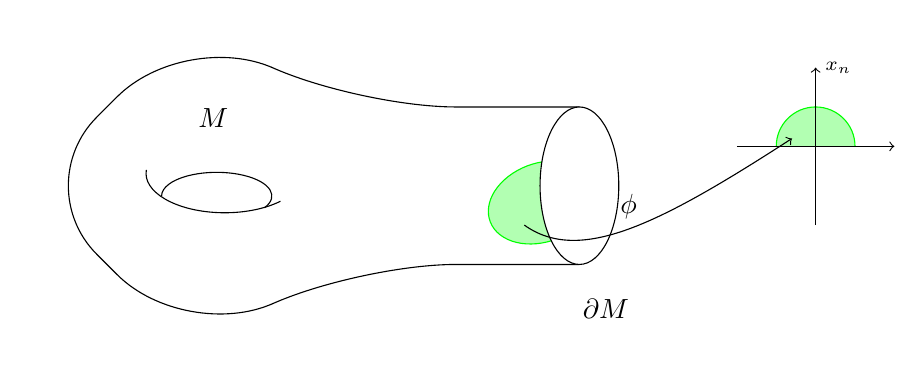
\begin{tikzpicture}
  \filldraw[color=green, fill=green!30, rotate around={20:(7, -0.5)}] (7, -0.5) arc (300:30:0.7 and 0.5);

  \filldraw[color=green, fill=green!30] (9.5,0.5) arc (180:0:0.5);
  \draw[->] (9, 0.5)--(11, 0.5);
  \draw[->] (10, -0.5)--(10, 1.5) node [right] {$\scriptstyle x_n$};

  \draw[rounded corners=35pt](7,-1)--(4.2,-1)--(2,-2)--(0,0) -- (2,2)--(4.2,1)--(7,1);
  \draw (1.5,0.2) arc (175:315:1cm and 0.5cm);
  \draw (3,-0.28) arc (-30:180:0.7cm and 0.3cm);
  \filldraw[color=black, fill=white] (7.5,0) arc (0:360:0.5cm and 1cm);
  \node (a) at (20:2.5) {$M$};
  \node (a) at (-12:7.5) {$\partial M$};

  \draw[->] (6.3, -0.5)..controls(7, -1)and(8, -0.5)..(9.7, 0.6) node [midway, above] {$\phi$};
\end{tikzpicture}
}
\end{center}

Lokalnie, na zbiorze mapowym $(U_\alpha,\phi)$ możemy funkcję spełniającą wymagania wyżej zadać przy pomocy funkcji wychodzącej z $\overline{U_\alpha}=\phi(U_\alpha)$
$$f_\alpha:\overline{U_\alpha}\to\R,\quad f(x_1,...,x_n)=x_n,$$
gdyż ostatnia współrzędna punktów z $\partial M$ jest zawsze zerowa (gdyż są one w $\partial H^n$). Stąd w prosty sposób dostajemy funkcję:
$$f_\alpha:U_\alpha\to\R,\quad f_\alpha=\overline{f_\alpha}\circ \phi$$
która lokalnie spełnia nasze wymagania. Nie możemy jednak w prosty sposób przełożyć lokalne $f_\alpha$ na funkcję $f:M\to\R$. 

\subsection{Lokalnie skończone rozdrobnienie}

Przypomnijmy definicje, które będą przydatne przy rozkładach jedności:

\begin{definition}[pokrycie lokalnie skończone] Pokrycie $\{A_\alpha\}$ podzbiorami przestrzeni topologicznej $X$ jest \important{lokalnie skończone}, jeśli dla każdego $p\in X$ istnieje otoczenie $U_p$ takie, że $U_p\cap A_\alpha\neq\emptyset$ tylko dla skończenie wielu $\alpha$.
\end{definition}

\begin{definition}[rozdrobnienie] Pokrycie $\{V_\beta\}$ przestrzeni $X$ zbiorami otwartymi nazywamy \important{rozdrobnieniem pokrycia} $\{U_\alpha\}$, jeśli każdy $V_\beta$ zawiera się w pewnym $U_\alpha$.
\end{definition}

Warto nadmienić, że relacja bycia rozdrobnieniem jest przechodnia.\marginpar{$\scriptstyle\{W_\gamma\}\prec\{V_\beta\}\prec\{U_\alpha\}\implies\;\implies\{W_\gamma\}\prec\{U_\alpha\}$} Będziemy oznaczać ją przez $\{V_\beta\}\prec\{U_\alpha\}$.

\begin{definition}[przestrzeń parazwarta] Przestrzeń topologiczna $X$ jest \important{parazwarta}, jeśli każde jej pokrycie $\{U_\alpha\}$ zbiorami otwartymi posiada lokalnie skończone rozdrobnienie $\{V_\beta\}$.
\end{definition}

Warto przypomnieć, że każda rozmaitość topologiczna jest parazwarta. \marginpar{Dowód: patrz Lee strona 36-37}Dowód tego lematu wykorzystuje w istotny sposób lokalną zwartość, czyli istnienie dla każdego punktu otoczeń prezwartych (po domknięciu zwartych). Własność ta została udowodniona na ćwiczeniach.

\begin{remark}\label{uwaga:2.4}
Rozdrobnienie wynikające z parazwartości rozmaitości topologicznych można z góry uznać za składające się z prezwartych zbiorów mapowych.
\end{remark}

\begin{proof}
Niech $\{U_\alpha\}$ będzie pokryciem $M$. Łatwo jest znaleźć rozdrobnienie $\{U'_\gamma\}\prec\{U_\alpha\}$ złożone ze zbiorów prezwartych mapowych. Wystarczy obraz każdego $U_\alpha$ w $\R^n$ pokryć zbiorami prezwartymi i wrócić z nimi na $M$. Z faktu, że rozmaitości są parazwarte dostajemy lokalnie skończone rozdrobnienie $\{V_\beta\}\prec\{U'_\gamma\}$, które z przechodności $\prec$ jest też rozdrobnieniem $\{U_\alpha\}$. Dodatkowo, każdy $V_\beta$ zawiera się w pewnym $U'_\gamma$, które były mapowe i prezwarte, więc i $V_\beta$ taki jest.
\end{proof}

\begin{remark}\label{uwaga:2.5}
  Niech $\{A_\alpha\}$ będzie lokalnie skończoną rodziną parazwartych podzbiorów rozmaitości $M$. Wtedy dla każdego $A_{\alpha_0}$ podrodzina
  $$\{A_\alpha\;:\;A_\alpha\cap A_{\alpha_0}\neq\emptyset\}$$
  jest skończona.
\end{remark}

\begin{proof}
  Załóżmy nie wprost, że dla pewnego $A_{\alpha_0}$ podrodzina $\{A_\alpha\;:\;A_\alpha\cap A_{\alpha_0}\neq\emptyset\}$ jest nieskończona. Możemy w takim razie wybrać z niej ciąg $A_{\alpha_i}$ oraz ciąg punktów $x_i\in A_{\alpha_i}\cap A_{\alpha_0}$. Ciąg $x_i$ ma punkt skupienia w pewnym $p\in cl(A_{\alpha_0})$. 

  Ponieważ $p$ jest punktem skupienia $x_i$, to dowolne otwarte otoczenie $U_p$ punktu $p$ zawiera nieskończenie wiele elementów $x_i$. W takim razie $U_p$ przecina się z nieskończenie wieloma zbiorami $A_\alpha$. Jest to sprzeczne z lokalną skończonościa $\{A_\alpha\}$.
\end{proof}

W uwadze \ref{uwaga:2.4} pokazaliśmy mapowość i prezwartość zbiorów z rozdrobnienia $\{V_\beta\}$ wynikającego z parazwartości rozmaitości topologicznych. Możemy teraz dodatkowo zapewnić sobie istnienie interesujących nas zbiorów zwartych:

\begin{remark}\label{wniosek:2.6}
  Niech $\{V_\beta\}$ będzie lokalnie skończonym rozdrobnieniem pokrycia $M$ składającym się ze zbiorów mapowych. Wtedy dla każdego $\beta$ istnieje zwarty zbiór $D_\beta\subseteq V_\beta$ taki, że
  $$\bigcup D_\beta=M$$
  to znaczy możemy wybrać "rozdrobnienie" przy pomocy zwartych zbiorów, które nadal pokrywa $M$.
\end{remark}
\begin{illustration}
  \draw (0, 0) circle (2cm);
  \draw (3, 0.4) circle (2cm);
  \node at (-1, 2) {$V_{\beta_1}$};
  \node at (4, 2.4) {$V_{\beta_2}$};
  \node[regular polygon, regular polygon sides=6, draw, inner sep=1.2cm] at (0, 0) {};
  \node[regular polygon, regular polygon sides=6, draw, inner sep=1.2cm, rotate=20] at (3, 0.4) {};
  \node at (-1, -0.8) {$D_{\beta_1}$};
  \node at (4, 1.3) {$D_{\beta_2}$};
\end{illustration}

\begin{proof}
  Ponieważ $V_\beta$ są zbiorami mapowymi, to o każdym z nich możemy myśleć jak o otwartym podzbiorze w $\R^n$ poprzez utożsamienie go z otwartym zbiorem $\overline{V_\beta}=\phi_\beta(V_\beta)$ dla mapy $(V_\beta, \phi_\beta)$.

  Każdy $V_{\beta_0}$ jest wstępującą suma mniejszych zbiorów $V_{\beta_0,k}$ dla $k\in\N$, które są otwarte i ich zwarte domknięcia zawierają się w $V_{\beta_0}$: $cl(V_{\beta_0,k})\subseteq V_{\beta_0}$. Możemy np. wybierać $V_{\beta_0,k}=B(x_0, k)\cap \{x\in V_{\beta_0}\;:\;d(x, V_{\beta_0^c}>\frac{1}{k}\}$, tzn. przekroje kul otwartych w $\R^n$ o środku w $x_0\in V_{\beta_0}$ i promieniu $k$ ze zbiorami tych $x\in V_{\beta_0}$, które są odległe od dopełnienia $V_{\beta_0}$ o co najmniej $\frac{1}{k}$.

  Niech teraz $V_{\beta_1},...,V_{\beta_m}$ będą zbiorami z $\{V_\beta\}$ niepusto krojącymi $V_{\beta_0}$. Jest ich skończenie na mocy \ref{uwaga:2.5}. Wówczas $V_{\beta_1},...,V_{\beta_m}$ wraz z wcześniej stworzonymi $V_{\beta_0,k}$ jest pokryciem zwartego zbioru $cl(V_{\beta_0})$. Możemy więc z niego wybrać skończone podpokrycie postaci: $V_{\beta_1},...,V_{\beta_m},...V_{\beta_0,k_0}$. Oznacza to, że zastępując w $\{V_\beta\}$ zbiór $V_{\beta_0}$ przez zbiór $V_{\beta_0, k_0}$ dostajemy nowe pokrycie $M$ z $cl(V_{\beta_0,k_0}\subseteq V_{\beta_0}$. Powtarzamy to induktywnie dla wszystkich $V_\beta$ i wybieramy pokrycie
  $$D_\beta=cl(V_{\beta, k}),$$
  które spełnia wymagania z uwagi.
\end{proof}

\begin{bbox}
Z uwag udowodnionych wyżej wynika więc, że dla dowolnego pokrycia otwartego $\{U_\beta\}$ rozmaitości topologicznej $M$ istnieje 
\begin{itemize}
  \item lokalnie skończone rozdrobnienie $\{V_\beta\}$ składające się ze zbiorów mapowych i parazwartych oraz
  \item rodzina $\{D_\beta\}$ zwartych podzbiorów $D_\beta\subseteq V_\beta$, która dalej pokrywa $M$.
\end{itemize}

To samo dotyczy też rozmaitości z brzegiem.
\end{bbox}

\subsection{Twierdzenie o rozkładzie jedności}

\begin{definition}[nośnik funkcji]Dla funkcji rzeczywistej $f:X\to \R$ określamy jej \important{nośnik} jako:
  $$\color{blue}supp(f):=cl(\{x\in X\;:\;f(x)\neq0\})$$
\end{definition}

\begin{fact}\label{fakt:2.8} [z $\R^n$] Dla dowolnego otwartego $\Omega\subseteq\R^n_+$ oraz dowolnego zwartego $D\subseteq \Omega$ istnieje gładka funkcja $f:\R^n\to \R$ taka, że:
  \begin{enumerate}
    \item $f\geq 0$
    \item $supp(f)\subseteq\Omega$
    \item $f(x)>0$ dla $x\in D$
  \end{enumerate}
\end{fact}

\begin{theorem}[o rozkładzie jedności] \emph{[O rozkładzie jedności]} Dla każdego otwartego pokrycia $\{U_\alpha\}$ rozmaitości gładkiej $M$ istnieje rodzina $\{f_i\}$ gładkich funkcji $f_i:M\to \R$ takich, że
  \begin{enumerate}
    \item $f_i\geq 0$
    \item dla każdego $i$ nośnik $supp(f_i)$ zawiera się w pewnym $U_\alpha$
    \item nośniki $\{supp(f_i)\}$ tworzą lokalnie skończone pokrycie $M$
    \item dla każdego $x\in M$ $\sum f_i(x)=1$ [suma ta jest skończona wokół każdego $x$ dzięki 3.]
  \end{enumerate}
\end{theorem}

\begin{proof}
Niech $\{V_j\}\prec\{U_\alpha\}$ będzie lokalnie skończonym pokryciem otwartym prezwartymi zbiorami mapowymi. Niech $D_j\subseteq V_j$ będą zbiorami zwartymi, które dalej pokrywają $M$ (na mocy \ref{wniosek:2.6}).

Niech $(V_j, \phi_j)$ będzie mapą na $M$ i niech
$$\overline{D}_j=\phi(D_j)\subseteq\phi_j(V_j)=\overline{V}_j$$
będzie zbiorem zwartym. Dzięki faktowi z $\R^n$ \ref{fakt:2.8} wiemy, że dla każdego $j$ istnieje gładka funkcja $\overline{h}_j:\R^n\to\R$ taka, że:
\begin{enumerate}
  \item $\overline{h}_j\geq 0$
  \item $supp(\overline{h}_j)\subseteq \overline{V}_j$
  \item $\overline{h}_j(x)>0$ dla $x\in D_j$.
\end{enumerate}
Zdefiniujmy teraz funkcję $h_j:M\to\R$ taką, że:
$$h_j(x)=\begin{cases}\overline{h}_j\circ\phi_j(x)&x\in V_j\\0&x\notin V_j\end{cases}$$
Żeby pokazać gładkość $h_j$, wystarczy pokazać jej gładkość na pewnym otoczeniu każdego punktu. 

Na otoczeniu punktów z $V_j$ funkcja jest oczywiście gładka jako złożenie dwóch funkcji gładkich. Dla $p\notin V_j$ istnieje otwarte otocznie $U_p$ które jest rozłączne z $supp(h_j)$, a więc jest otwartym otoczenie na którym $h_j$ jest stale równe zero. Taka funkcja jest oczywiście gładka.

Niech teraz $h(x)=\sum_jh_j(x)$. Jest to dobrze określona definicja, gdyż $supp(h_j)$ tworzą rodzinę lokalnie skończoną (bo $\{V_j\}$ taka jest). Z lokalnej skończoności nośników wynika, że $h$ jest gładka na $M$.

Dostajemy też $h(x)>0$, bo $D_j$ pokrywają całe $M$, a więc dla każdego $x\in M$ istnieje $i$ takie, że $x\in D_i$, a więc $h_i(x)>0$.

Określmy $f_j(x)=\frac{h_j(x)}{h(x)}$. Wiemy, że $f_j:M\to\R$ jest gładka na $M$, $supp(f_j)=supp(h_j)\subseteq V_j$, więc rodzina $\{supp(f_j)\}$ jest lokalnie skończona i każdy $supp(f_j)$ zawiera się w pewnym $U_\alpha$. Wreszcie mamy
$$\sum f_j(x)=\sum\frac{h_j(x)}{h(x)}=\frac{\sum h_j(x)}{h(x)}=\frac{\sum h_j(x)}{\sum h_j(x)}=1$$
dla każdego $x\in M$.
\end{proof}

\begin{definition}[rozkład jedności] Rodzina funkcji $\{f_j\}$ jak w dowodzie twierdzenia wyżej jest nazywana \important{rozkładem jedności} wpisanym w pokrycie $\{U_\alpha\}$.
\end{definition}

\subsection{Zastosowania rozkładów jedności}

Zazwyczaj rozkłady jedności służą do konstruowania gładkich funkcji, które są określone na całym $M$ i spełniają pewne wymagania. Z pomocą rozkładów jedności będziemy też "globalizować" inne obiekty na rozmaitościach, np. pola wektorowe, metryki Riemanna czy formy różniczkowalne.

\begin{example}
\item Niech $F_1,F_2$ będą domkniętymi rozłącznymi podzbiorami gładkiej rozmaitości $M$. Wówczas istnieje gładka funkcja $f:M\to[0,1]$ taka, że 
  $$f\restriction F_1\equiv 1$$ 
  oraz $f\restriction F_2\equiv 0$.

  \begin{proof}
    Niech $U_i=M\setminus F_i$, wtedy $\{U_1,U_2\}$ jest pokryciem $M$. Niech $\{f_i\}$ będzie rozkładem jedności wpisanym w $\{U_1,U_2\}$. Określmy 
    $$f(x)=\sum_{supp(f_j)\subseteq U_2}f_j(x).$$

    Weźmy $x\in F_1$, wtedy wszystkie nośniki $supp(f_i)$ zawierające $x$ zawierają się w $U_2$, zatem dla takich $x$ jest
    $$f(x)=\sum f_i(x)=1$$

    Jeśli $x\in F_2$, to nośniki $supp(f_i)$ zawierające $x$ nie mogą zawierać się w $U_2$. W takim razie $f(x)=0$.
  \end{proof}
\item Rozważmy istnienie gładkiej funkcji $f:M\to\R$ takiej, że 
  $$f(p)=\begin{cases}=0&p\in\partial M\\>0&p\in Int(M)\end{cases}$$

  Niech $\{U_\alpha\}$ będzie dowolnym pokryciem zbiorami mapowymi, a $f_\alpha:U_\alpha\to\R^n$ będą lokalnie gładkimi funkcjami takimi, że
  $$f_\alpha=\begin{cases}\overline{f}_\alpha\circ\phi_\alpha&U_\alpha\cap\partial M\neq\emptyset\\1&U_\alpha\cap\partial M=\emptyset\end{cases}$$
  gdzie $\overline{f}_\alpha:\overline{U}_\alpha\to\R$ jest zdefiniowane jako
  $$\overline{f}_\alpha(x_1,...,x_n)=x_n.$$

  Niech $\{h_\beta\}$ będzie rozkładem jedności wpisanym w $\{U_\alpha\}$. Dla każdego $\beta$ wybieramy $\alpha(\beta)$ takie, że $supp(h_\beta)\subseteq U_{\alpha(\beta)}$. Definiujemy $h_\beta':M\to\R$ przez
  $$h_\beta'=h_\beta\circ f_{\alpha(\beta)}.$$
  Wtedy $h_\beta'$ jest gładkie oraz $supp(h_\beta')\subseteq supp(h_\beta)$, więc rodzina nośników $\{supp(h_\beta')\}$ jest lokalnie skończona.

  Zdefiniujmy teraz
  $$f(x)=\sum h_\beta',$$
  które z lokalnej skończoności nośników $\{supp(h_\beta'\}$ jest dobrze określone.

  \begin{itemize}
    \item $p\in\partial M$, to dla każdego $\beta$ $h_\beta'(p)=0$, więc $f(p)=0$.
    \item $p\in Int(M)$, to wtedy istnieje $\beta$ takie, że $h_\beta(p)>0$, a ponieważ dla $\gamma\neq\beta$ $h_\gamma'(p)\geq0$, to $f(p)>0$.
  \end{itemize}
\item Dla dowolnego $A\subseteq M$ domkniętego oraz $A\subseteq U\subseteq M$ otwartego istnieje \marginpar{Po angielsku taka funkcja nazywa się \emph{bump function}}funkcja $f:M\to\R$ taka, że dla $x\in A$ $f(x)=1$ oraz $supp(f)\subseteq U$.
  
  \begin{proof}
    Niech $U_1=U$ oraz $U_2=M\setminus A$, zbiory te pokrywają całe $M$. Niech $h_1,h_2$ będzie rozkładem jedności wpisanym w to pokrycie. Wtedy funkcja $h_1$ ma poszukiwane własności, bo dla $x\in A$ mamy $h_2(x)=0$, więc $1=h_1(x)+h_2(x)=h_1(x)$.
  \end{proof}
\item Funkcja $f:M\to\R$ jest nazywana \emph{exhaust function}, jeśli dla każdego\marginpar{Dowód istnienia to wniosek 2.28 z Lee.} $c\in\R$ $f^{-1}((-\infty,c])$ jest zwartym podzbiorem $M$. Kiedy idąc po liczbach naturalnych $n$ rozpatrujemy $f^{-1}((-infty, n])$, to po drodze zahaczamy o wszystkie zwarte zbiory w $M$, stąd też nazwa. Dowód istnienia exhaust function korzysta z rozkładów jedności $\{h_i\}$ wpisanych w dowolne pokrycie prezwartymi zbiorami oraz funkcji $f(x)=\sum_{j\geq 1}j\cdot\phi_j(x)$.
\end{example}

\subsection{Alternatywna wersja twierdzenia o rozkładzie jedności}

\begin{theorem}
  Dla dowolnego otwartego pokrycia $\{U_\alpha\}_{\alpha\in A}$ rozmaitości gładkiej $M$ istnieje rodzina $\{f_\alpha\}$ gładkich funkcji $f_\alpha:M\to\R$ takich, że
  \begin{enumerate}
    \item $f_\alpha\geq0$
    \item $supp(f_\alpha)\subseteq U_\alpha$
    \item nośniki $\{supp(f_\alpha)\}$ tworzą lokalnie skończone pokrycie $M$ [czyli wiele spośród $f_\alpha$ jest zerowych]
    \item dla każdego $x\in M$ $\sum f_\alpha(x)=1$
  \end{enumerate}
\end{theorem}

\begin{proof}
  Znowu szkic dowodu za pomocą wyjściowej wersji twierdzenia.

  Rozważmy rodzinę $\{f_j\}_{j\in J}$ jak w wyjściowej wersji twierdzenia. Dla każdego $j\in J$ wybieramy $\alpha(j)\in A$ takie, że $supp(f_j)\subseteq U_{\alpha(j)}$. Zdefiniujmy
  $$f_\alpha=\sum_{j:\alpha(j)=\alpha}f_j.$$
  Z lokalnej skończoności nośników $supp(f_j)$ wiemy, że $f_\alpha$ również jest funkcją gładką. Warunek $4$ zachodzi w sposób oczywisty, tak samo warunek $1$.

  Warunki $2$ i $3$ w łatwy sposób wynikają z obserwacji, że dla dowolnej lokalnie skończonej rodziny podzbiorów $P_t$ w przestrzeni $X$, $cl(\bigcup P_t)=\bigcup cl(P_t)$.
\end{proof}
